\chapter{Praca własna}
Proces twórczy został podzielony na dwa główne etapy: projektowanie i~implementację. Ponieważ tworzenie gry wymaga przygotowania oraz doboru odpowiedniego środowiska, etapy te zostały poprzedzone analizą problemu oraz burzą mózgów na której zarysowały się wstępne wymagania funkcjonalne. Zdefiniowane zostały również główne wymagania pozafunkcjonalne, takie jak docelowa platforma obsługująca grę. W celu zapewnienia spójnej wizji gry wśród członków zespołu, postanowiono skonstruować dokument, zawierający opis wszystkich decyzji podjętych podczas tworzenia projektu oraz wyjaśnienia dotyczące wszystkich wymagań funkcjonalnych oraz pozafunkcjonalnych -- Game Design Document (GDD), stanowiący jednocześnie załącznik~1 do niniejszej pracy.  Pomysły zebrane podczas burzy mózgów zostały poddane wnikliwej analizie, co pozwoliło na stworzenie spójnej wersji projektu. 

\section{Projektowanie}
Projektowanie jest bardzo ważnym etapem prac nad każdym projektem informatycznym. Pozwala uspójnić wizję gry w~zespole oraz zdefiniować zadania, które będą wykonywane podczas implementacji. Dlatego dobrze, gdy na tym etapie pracy w proces twórczy zaangażowany jest każdy członek zespołu. 

Istnieje wiele sposobów na projektowanie gry komputerowej. Podejściem, które ułatwia stworzenie gry, która bawi, jest projektowanie zorientowane na gracza. Zgodnie z~charakterystyką przedstawioną w~\cite{Adams:pgp}, stosując tę metodę, twórcy powinni wyobrazić sobie typowego gracza, a~więc osobę, dla której ta gra jest tworzona. Aby użytkownik był zadowolony, należy zapewnić mu rozrywkę -- jest to podstawowa funkcja gry. W~tym celu należy utożsamić się z~graczem. Pozwoli to wybrać funkcje, które uczynią grę atrakcyjną.

Istotnym elementem tworzenia projektu gry jest wnikliwa analiza wymagań funkcjonalnych oraz uszeregowanie ich według wagi. Każdy z członków zespołu posiadał własną wizję gry. Połączenie ich wszystkich zaowocowało spójnym projektem, opisanym w~załączniku~1 -- GDD. 

Aby zapewnić, że projekt będzie spójny, konieczne jest stworzenie dokumentów projektowych. Powstrzymuje to programistów przed puszczaniem wodzy fantazji i~tworzeniem funkcjonalności niezgodnych z projektem. 

Na tym etapie przydatna okazała się nie tylko teoretyczna wiedza na temat tworzenia zaawansowanych projektów informatycznych, ale przede wszystkim doświadczenia innych twórców gier, które zespół poznał przy okazji udziału w~konferencjach takich jak Zjazd Twórców Gier (ZTG) czy World of Gamedev Knowledge (WGK). Zdobyto wiedzę potrzebną między innymi do stworzenia poziomów ciekawych dla graczy, wyboru funkcjonalności nie wymagających skomplikowanych i~często zawiłych implementacyjnie elementów (co często powoduje błędy i~trudności w~dalszym rozwoju projektu), jednocześnie będących skomplikowanymi z~punktu widzenia gracza. 

Dobrą praktyką przy tworzeniu gry jest również częste testowanie graficznego interfejsu użytkownika, jego czytelności i~łatwości użycia kluczowych funkcji w~ferworze walki. Pozwala to zaprojektować interfejs przyciągający wzrok oraz funkcjonalny. Projektując HUD [ang. \emph{Head-Up Display}], a~więc wszystkie istotne w~trakcie rozgrywki wskaźniki, mapkę, poziom życia; postanowiono rozmieścić interesujące dla graczy informacje analogicznie do popularnych gier z~gatunku strzelanek. Jest to dla nich atrakcyjne, ponieważ nie muszą zmieniać swoich przyzwyczajeń by sprawdzić poziom życia. 

Jednak projektowanie to nie tylko uspójnienie rozgrywki, ale również specyfikacja dotycząca środowiska, w~którym gra powstanie. W tym celu należało wybrać odpowiednie narzędzia, co zostało opisane w~Rozdziale 3: Przegląd narzędzi. 

\subsection{Projekt silnika graficznego}

W ramach pracy jako pierwsze przetestowano podejście z~tworzeniem własnego silnika graficznego w~języku C++. Jak zostało wspomniane w~poprzednim rozdziale, tworzenie tego rodzaju oprogramowania wymaga pewnej określonej wiedzy dotyczącej zarówno architektury silników~graficznych i~inżynierii oprogramowania, jak i~grafiki komputerowej oraz Microsoft DirectX API. Jako że wiedza teoretyczna wraz z podstawowymi pojęciami zostały zarysowane w rozdziale 2., tutaj opisane zostaną kwestie dotyczące architektury silnika oraz usprawnień, które mogłyby zostać wprowadzone w~przyszłości.\\

W silniku graficznym można zasadniczo wydzielić 3 podstawowe składowe:
\begin{itemize}
\item renderer - przeprowadza proces renderingu, tj. generowania grafiki,
\item menedżer obiektów - zawiera listę obiektów i/lub listę ich grup,
\item menedżer zasobów - odpowiada za alokację i zwalnianie zasobów takich jak tekstury, dźwięki itp.
\end{itemize}

W ramach menedżera obiektów zastosowano wzorzec kompozyt ze względu na jego idealne dopasowanie do problemu.
Jak widać każda z~tych składowych może stanowić pewną jednostkę (ang. \emph{entity}) budującą system - w~tym wypadku system graficzny (wyróżnia się również na przykład systemy fizyki). Jednostki można również podzielić na mniejsze komponenty, które można dynamicznie dodawać i~usuwać w trakcie działania - podejście takie zgodne jest wzorcem \emph{Entity-Component-System}. Jak zauważono podczas testowania opisywanego oprogramowania, poza wygodą oraz nowymi możliwościami rozwoju wykorzystanie dynamicznych komponentów wprowadza także narzut czasowy ze względu na wykorzystanie metod wirtualnych oraz nieoptymalne wykorzystanie pamięci podręcznej procesora. W~tym wypadku możliwym usprawnieniem mogłoby być budowanie aplikacji z~komponentów w~edytorze, a~następnie generowanie ''stałych'' klas i~kompilowanie zmodyfikowanego w~ten sposób kodu do pliku wykonywalnego, który mógłby być dystrybuowany jako gotowa aplikacja.\\
Nieoptymalne wykorzystanie pamięci podręcznej procesora dotyczy nie tylko wykorzystania komponentów, gdyż jest wąskim gardłem większości zarówno amatorskich jak i~profesjonalnych silników graficznych. W~celu zniwelowania tego problemu można utworzyć pewien stały obszar pamięci (w~języku C++ w~wersji 11. w tym celu wykorzystać można operator \emph{placement new}) i~utworzyć pulę obiektów, w~ramach której mogłyby one być używane ponownie bez konieczności zwalniania zajmowanej przez nie pamięci.\\
Ostatnim usprawnieniem, które można byłoby wprowadzić celem zwiększenia efektywności procesu renderingu jest wielowątkowość, która jednak wymagałaby wprowadzenia synchronizacji między wątkami aplikacji (np. zamki) oraz użycia metod DirectX obsługujących wielowątkowość (np. operować na opóźnionym kontekście urządzenia). Jej użycie utrudniałoby też skuteczną naprawę błędów ze względu na brak możliwości odpluskwiania kodu w środowisku Microsoft Visual Studio, w którym tworzone było to oprogramowanie.\\
Dla silnika została napisana i wygenerowana z wykorzystaniem aplikacji Doxygen dokumentacja, jednak ze względu na swoją objętość (150 stron) nie została tutaj załączona.
% dodawać wykaz klas, przestrzeni nazw i kod źródłowy + dokumentację w pdf?
% dodać do literatury tekst o EntityComponentSystem + o deferred shading i tutoriale z animacji

\subsection{Modele 3D i animacje}

Jak wspomniano w~rozdziale dotyczącym narzędzi, do stworzenia modeli i~animacji wykorzystano narzędzie 3D Studio MAX firmy Autodesk. Ponieważ w~wypadku modeli 3D -- podobnie jak w przypadku grafik -- jest trudny do uporządkowania w ramach podejścia inżynierskiego, postanowiono dokonywać na modelu małych przyrostów, rozpoczynając ten proces od utworzenia pojedynczej powierzchni płaskiej i~wyprowadzeniu z niej połowy modelu, a~następnie odbiciu jej względem odpowiedniej osi.\\
Animacje z kolei wykonane zostały z wykorzystaniem Character Animation Toolkit -- zestawu narzędzi wbudowanego w 3DS MAX i pozwalającego na o wiele łatwiejszą i~uniwersalną animację modeli, w przeciwieństwie do domyślnych funkcji animacji szkieletowej tego programu. Dla modelu utworzono szkielet (Rys. \ref{max_skeleton}), a~następnie wykorzystano gotowy zestaw animacji, który z kolei został drastycznie zmieniony na potrzeby pracy (jest to jedyna możliwość tworzenia animacji w CAT, która pozwala na pewną swobodę jednocześnie dając pewien niezerowy punkt wyjściowy).

Gotowy model z zaaplikowaną animacją chodu przedstawiony został na Rys. \ref{max_animated}.

\subsection{Projekt poziomu}

Do stworzenia poziomu wykorzystano środowisko Unreal Development Kit (w skrócie UDK), do którego zaimportowano wcześniej stworzone modele. Niewątpliwą zaletą UDK jest możliwość szybkiego stworzenia poziomu poprzez przenoszenie obiektów z panelu edytora prosto na tworzoną mapę. A także oprogramowanie wydarzeń występujących na niej zgodnie z zasadami programowania wizualnego, za pomocą komponentów, układanych obok siebie i łączonych liniami z wykorzystaniem interfejsu graficznego.

W tworzeniu poziomu istotne jest jego umiejscowienie w realiach rozgrywki. Poziom powinien być powiązany z fabułą i światem przedstawionym. W związku z tym istotne było określenie czasu i miejsca akcji. Ponieważ podczas burzy mózgów ustaliliśmy, że fabuła gry będzie polegać na potyczkach żelków to istotne stało się dopasowanie miejsca aby zwiększyć immersję a co za tym idzie przyjemność z gry. W związku z tym, że żelki są jedzeniem a jedzenie jest powiązane z kuchnią, oczywisty stał się wybór tego pomieszczenia jako miejsce starcia. Stworzono, więc wstępny projekt poziomu. Stworzono go w programie Gimp. Jego celem był wstępny zarys, zorientowanie się jak co powinno wyglądać a także przekazanie informacji, jakie tekstury wykonać. Wstępny projekt został stworzony szybko i zawiera jedynie kontury obiektów, gdyż służy głównie do zorientowania się w koniecznych do stworzenia modelach oraz skonsultowania z członkami grupy rozmieszczenia elementów w celu zwiększenia przyjemności z gry, gdyż każdy z nich grał wcześniej w tego typu gry i ma doświadczenie z gry na wielu planszach i może pomóc lepiej zaprojektować poziom. Istotną bowiem sprawą w tworzeniu poziomu jest takie jego zaprojektowanie by był sprawiedliwy i dawał graczom dużo możliwości, różnego poprowadzenia rozgrywki. Dlatego obmyślono stworzenie stołu po którym gracz będzie mógł się wspinać i zaskakiwać przeciwników z wysokości a także porozrzucanie po pomieszczeniu (w tym przypadku kuchni), obiektów służących jako osłony, dzięki czemu łatwiej będzie się schować i zaskoczyć oponenta, tym samym zmniejszając wielkość otwartych przestrzeni, które na podstawie doświadczeń grupy w zbyt dużej liczbie obniżają przyjemność płynącą z grania poprzez zmniejszenie możliwych taktyk.

Następnym krokiem było stworzenie poziomu w edytorze. W tym celu wykorzystano gotowe modele i zaprojektowano mieszkanie 3 pokojowe z korytarzem. Zwiększenie liczby pomieszczeń miało na celu zwiększenie możliwych punktów startu a także oddalenie ich od siebie w celu nie natrafienia od razu na przeciwnika. W innym przypadku mogłoby wyniknąć niezadowolenie z rozgrywki, z powodu różnic komputerów biorących udział w rozgrywce, ładują one poziom w różnym czasie, więc możliwe są drobne różnice czasu. A ponieważ strzelanki to gatunek gier szybkich, nawet niewielka różnica może zadecydować o zwycięstwie w potyczce. Dodatkowo w poziomie uwzględniono możliwość wspinania się (oprócz stołów) na niektóre obiekty, a także wykorzystanie kilku szklanych przeszkód (niezależnie od normalnych przeszkód), przez które widać przeciwnika, a których nie można zniszczyć. Umożliwia to bowiem ukazanie możliwości Directx 11 a także urozmaica rozgrywkę.

Poziom został stworzony z myślą o grze wieloosobowej w trybie każdy na każdego, w związku z tym nie było potrzeby tworzenia specjalnych sektorów dla każdej drużyny, a co za tym idzie jest więcej punktów startowych i w kolejnych rozgrywkach możliwe jest wylosowanie innego, więc konieczne są modyfikacje taktyki i sposobu gry, wynikające z innego otoczenia startowego.

\section{Implementacja}

\subsection{Wykorzystanie technologii DirectX 11 w~UDK}

W ramach wsparcia DirectX 11, Unreal Development Kit obsługuje trzy opisane w~rozdziale teoretycznym techniki: rozproszenie podpowierzchniowe (subsurface scattering), deferred shading (znany także jako \emph{deferred rendering}) oraz rozszerzenie techniki głębi ostrości o~nazwie \emph{bokeh depth of field} (bokeh [od jap. \emph{boke} w romaji - rozmycie] to efekt rozmycia obrazu z pewnym zniekształceniem, którego kształt zależy od kształtu soczewki - Rys. \ref{bokeh_example}).\\

Technikę rozproszenia podpowierzchniowego wykorzystano w~celu stworzenia materiału, z~którego wykonany jest gracz. Zgodnie z~\cite{udk_sss}, aby tego dokonać, należy najpierw aktywować opcję ''Enable Subsurface Scattering'' w~zakładce ''D3D11'', a~następnie ustawić wymagane parametry, czyli kolor światła rozproszonego (SubsurfaceInscatteringColor), kolor światła pochłoniętego (SubsurfaceAbsorptionColor) oraz promień rozproszenia (SubsurfaceScatteringRadius). W celu uzyskania realistycznego wyglądu materiału, zmieniono także metodę mieszania na ''BLEND\_Translucent'' (pozwala to uzyskać materiał półprzezroczysty, w przeciwieństwie do domyślnej wartości BLEND\_Opaque). Na Rys. \ref{sss_material_editor} przedstawiony został widok materiału w edytorze, zaś na Rys. \ref{sss_material_example} - przykłady jego użycia.\\

Z~\cite{udk_bokeh_dof} wynika, iż użycie techniki Bokeh Depth of Field wymaga jedynie utworzenie odpowiedniej tekstury (w~niniejszej pracy użyto tekstury pięciokąta foremnego pokazanej na~Rys. \ref{bokeh_texture}) oraz ustawienia wartości ''DepthOfFieldType'' na ''BokehDOF'' w efekcie końcowym procesu renderingu (etap ten nie ma swojej nazwy w języku polskim, natomiast oryginalnie nosi nazwę \emph{post-processing}).\\

Ostatnia funkcjonalność DirectX 11, czyli Deferred Shading jest włączona domyślnie gdy używany jest renderer DX11 \cite{udk_deferred_shading}, dzięki czemu nie było koniecznym włączenie tej opcji ręcznie.

\begin{figure}
\begin{center}
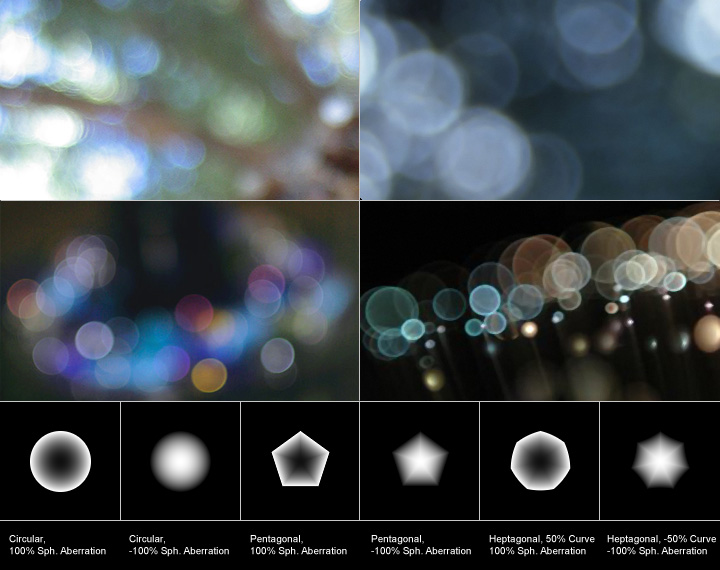
\includegraphics[scale=0.4]{figures/bokeh.jpg}
\captionsource{Rodzaje bokeh}{http:\/\/www.dofpro.com\/gallery\/dofpro\_spherical\_aberrations.jpg}
\label{bokeh_example}
\end{center}
\end{figure}

\begin{figure}
\begin{center}
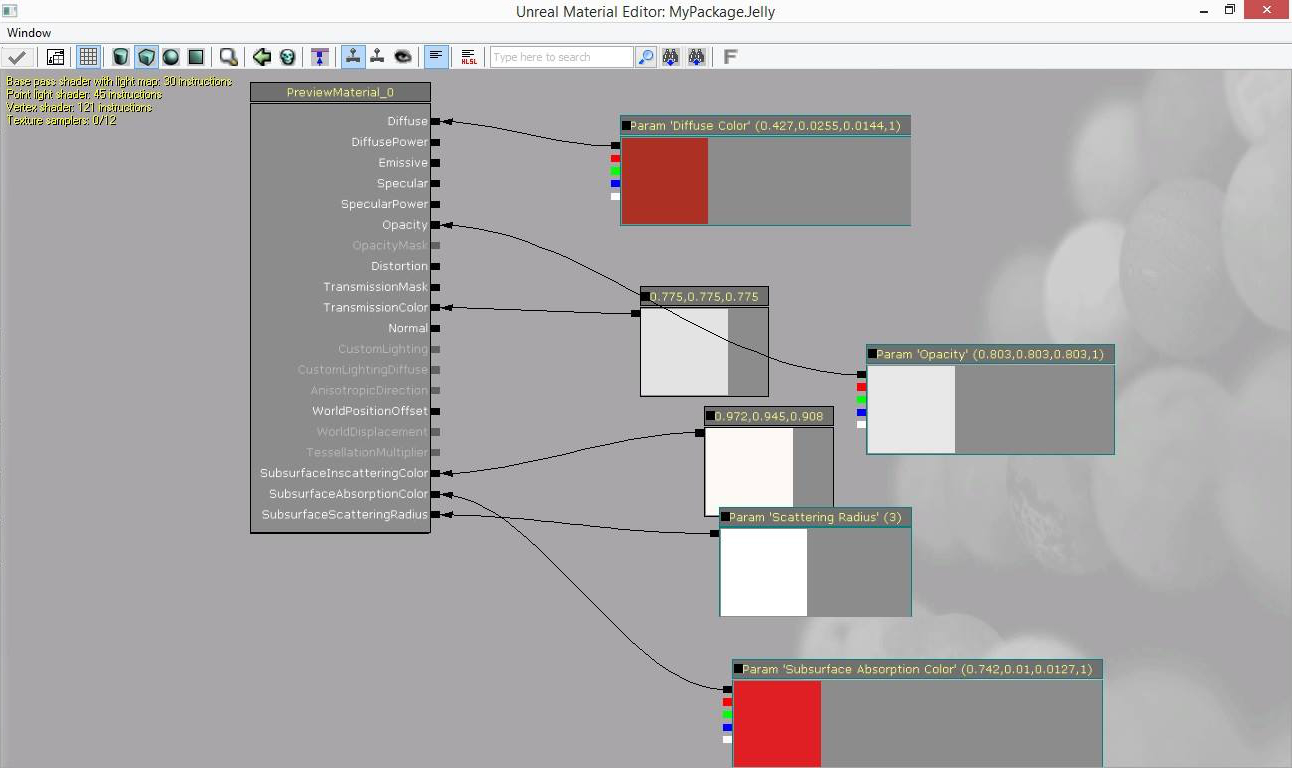
\includegraphics[scale=0.3]{figures/sss_material_editor.jpg}
\caption{Materiał wykorzystujący rozproszenie podpowierzchniowe w edytorze}
\label{sss_material_editor}
\end{center}
\end{figure}

\begin{figure}
\begin{center}
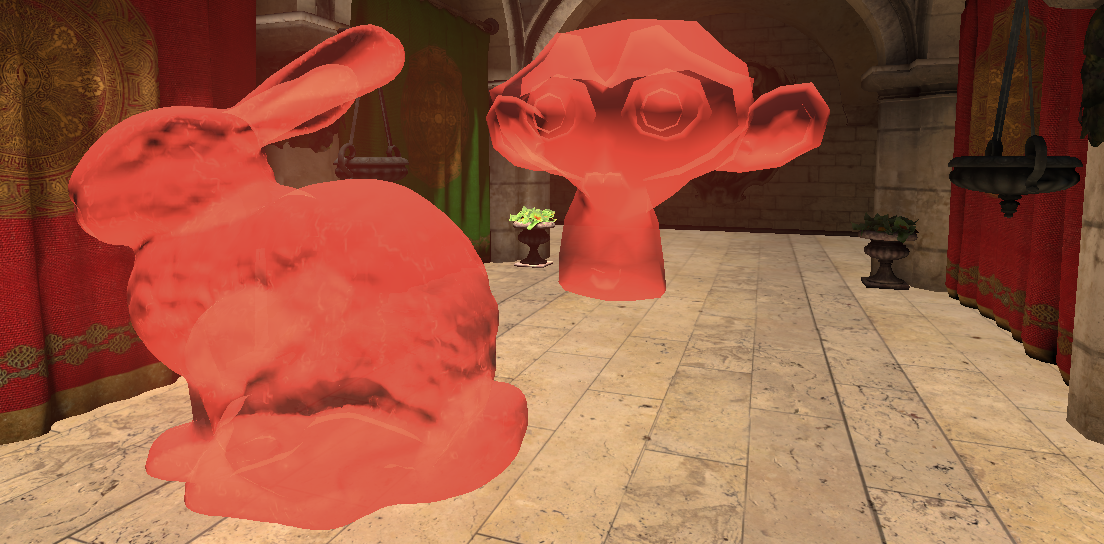
\includegraphics[scale=0.4]{figures/jelly_material.png}
\caption{Przykłady użycia materiału wykorzystującego rozproszenie podpowierzchniowe}
\label{sss_material_example}
\end{center}
\end{figure}

\begin{figure}
\begin{center}
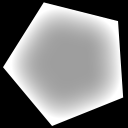
\includegraphics[scale=0.6]{figures/T_Bokeh_Pentagon.png}
\caption{Tekstura bokeh użyta w tworzonej grze}
\label{bokeh_texture}
\end{center}
\end{figure}

\subsection{Skryptowanie}

Jednym z elementów pracy własnej jest oskryptowanie działań, obiektów, mechanizmów rządzących rozgrywką. Sama implementacja skryptów odbywała się w języku UnrealScript, który jest językiem skryptowym, stworzonym na potrzeby Unreal Engine. Język ten jest zorientowany obiektowo i niewrażliwy na wielkość liter. Użyto tego języka do stworzenia kodu odpowiedzialnego za wykorzystanie kamery trzecioosobowej, kontrolę gracza oraz stworzenie nowych rodzajów broni, które zostały wykorzystane w rozgrywce wieloosobowej.

\subsection{Zarządzanie projektem}
W~celu sprawnej organizacji pracy w~zespole wykorzystano metody zarządzania projektami. Uspójnienie projektu gry podczas fazy projektowania pozwoliło na zdefiniowanie i~wyspecyfikowanie zadań, realizowanych podczas implementacji. Znając liczbę zadań, można było podzielić projekt na kolejne przyrosty. Projekt miał być realizowany z~wykorzystaniem metod zwinnych. Trudnością w~wykorzystaniu typowej zwinnej metody, takiej jak programowanie ekstremalne czy Scrum okazał się charakter projektu, będącego pracą dyplomową. Z~tego względu narzucony został ostateczny termin ukończenia produktu. Jest to sprzeczne z manifestem zwinności, dlatego zdecydowano się na inne rozwiązanie.

Początkowo użyto modelu kaskadowego. Jego zaletą jest sekwencyjność, pozwalająca oddzielić procesy analizy problemu, projektowania, implementacji oraz testowania i~późniejszego utrzymania projektu, co przedstawiono na Rys. \ref{waterfall}. Metoda Waterfall, wykorzystująca ten model, nie jest jednak pozbawiona wad. Dotyczą one głównie dużych projektów, a~więc nie miały miejsca w~przypadku oprogramowania tworzonego w~czteroosobowym zespole programistów. Korzystając z~tej metody oszczędza się czas na planowaniu. Jak opisano w~\cite{Kaczor:Scrum}, faza ta zajmuje zaledwie 25\% czasu pracy nad projektem. Rezultat końcowy zostaje ustalony jeszcze przed rozpoczęciem implementacji, podobnie jak poszczególne przyrosty implementacji. Każdy przyrost miał trwać 2 tygodnie i~zawierał określone zadania. Rezultatem końcowym był produkt posiadający wartość biznesową, w~tym przypadku - w~pełni działająca gra. Co istotne, wartość biznesową produkt miał zyskać dopiero w~przedostatnim przyroście. 

\begin{figure}
\begin{center}
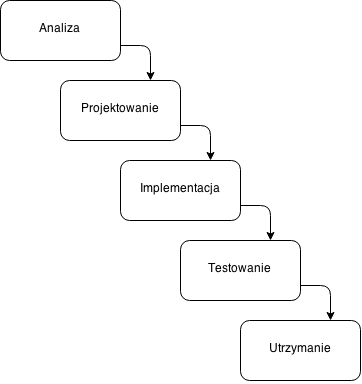
\includegraphics[scale=0.4]{figures/waterfall.png}
\caption{Model kaskadowy}
\label{waterfall}
\end{center}
\end{figure}

Problemem w~wykorzystaniu modelu kaskadowego są błędy, wykryte podczas fazy testowania. Ponieważ w~momencie rozpoczęcia testów cały produkt jest już zaimplementowany, poprawka może spowodować powstanie kolejnych błędów. Może jednak się zdarzyć, że błąd powstał na etapie projektowania, w~takim przypadku należy powtórzyć tę fazę, jak również całą fazę implementacji. Powoduje to wydłużanie czasu realizacji oraz wzrost kosztów wytworzenia produktu.

W~niedługim czasie po zaplanowaniu prac nad projektem okazało się, że metoda ta nie jest wystarczająca, zaczęło się pojawiać opóźnienie w~pracach, które mogło spowodować pogorszenie jakości produktu. Zdecydowano się więc skorzystać z~metod zwinnych. Metodyki Agile charakteryzują się stałą jakością, a~sterowane są zakresem. W~omówionej wcześniej metodzie Waterfall zakres był stały, zmieniała się jedynie jakość, a~chęć utrzymania wysokiej jakości powodowała opóźnienie względem planu. 

Ostatecznie zastosowano metodykę zwinną zbliżoną do metody Feature-Driven Development, wplatając w~nią elementy metodologii Scrum. Zadania podzielono na część dotyczącą rozpoznania danego zagadnienia i~część implementacyjną. 

W~części dotyczącej rozpoznania zastosowano cykl PDCA (\emph{Plan -- Do -- Check -- Act}), stworzony przez Williama Edwardsa Deminga. Pierwszy etap cyklu -- planowanie -- polegało na zapoznaniu się z~opisem wybranej funkcjonalności, zawartym w~Game Design Document. Następnie, w~fazie wykonania, zbierano informacje na temat możliwości implementacji funkcjonalności wykorzystując UDK oraz próbowano stworzyć wybraną funkcję. W~trzeciej fazie sprawdzano czy zaimplementowana wersja funkcji odpowiada założeniom projektu. Jeśli wynik był pozytywny, funkcjonalność została wybierana do wykonania w~kolejnym przyroście.

Realizowane były tygodniowe sprinty (przyrosty). Każdy sprint rozpoczynał się spotkaniem zespołu, na którym omówiono pozostałe zadania oraz zaplanowano jakie funkcjonalności będą implementowane w~kolejnym przyroście. W~efekcie udało się zachować jakość wykonania oraz zakończyć prace przed upływem niezmiennego terminu ukończenia, modyfikując nieznacznie zakres dostępnych funkcjonalności. Zespół tworzący grę był wskroś-funkcjonalny, co oznacza, że członkowie zespołu wykonywali zadania dotyczące różnych zagadnień. Począwszy od tworzenia prostych modeli 3D po skryptowanie. Jest to cecha charakterystyczna metody Scrum. Z~kolei sposób planowania kolejnych przyrostów, a~więc planowanie ze względu na funkcjonalność, zaczerpnięto z~metody Feature-Driven Development. 

Na koniec każdego przyostu otrzymywano prototyp posiadający pewną funkcjonalność. Jeśli funkcjonalność działała prawidłowo podczas testów, dołączano ją do głównego prototypu, który z~każdym przyrostem stawał się bardziej funkcjonalny, aż w~końcu stał się wersją produkcyjną. Ze względu na wcześniejszy nieudany eksperyment z~metodą Waterfall wartość biznesową projekt zyskał dopiero po kliku przyrostach. Oznacza to, że pierwsze efekty nie były satysfakcjonujące, jednak prezentowały postęp prac. 

\begin{figure}
\begin{center}
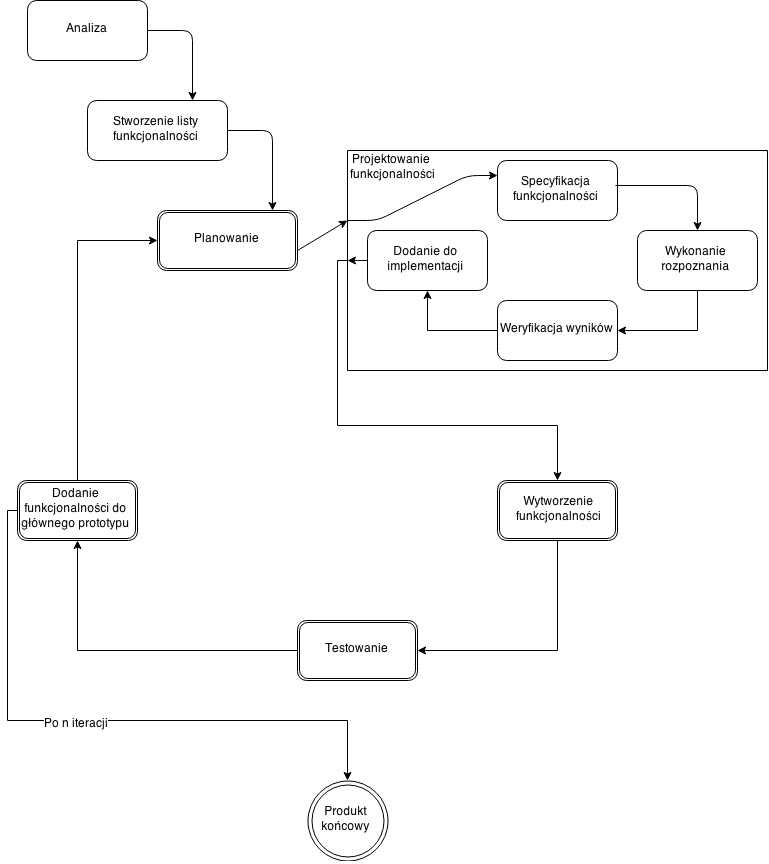
\includegraphics[scale=0.4]{figures/ujelly_phases.png}
\caption{Etapy procesu wytwórczego gry przy wykorzystaniu metody Feature-Driven Development i~cyklu PDCA}
\label{ujelly_phases}
\end{center}
\end{figure}

Trzy główne fazy procesu wytwarzania gry, występujące w~modelu kaskadowym, a~więc: projektowanie, implementacja i~testowanie, w~metodach zwinnych są wykonywane w~każdym sprincie, co znacznie zmniejsza ryzyko powstania krytycznych błędów po zaimplementowaniu całego produktu. W~przypadku wykorzystania Feature-Driven Development proces naprawy błędów również obarczony jest mniejszym ryzykiem czasowym. Zwłaszcza, gdy błąd powstał na etapie projektowania danej funkcjonalności. W~skrajnym przypadku, wadliwa funkcjonalność nie trafi do głównego produktu.
